To check the analytical model, we calculated the values of the complex refractive index $m$, using resonance conditions from first order approximation at $\lambda_{10} = 83$ nm, $ka = 0.7$: $m = 1.851i$. The complex refractive index is purely imaginary, since the collision coefficient $v_e$ in the case under consideration is somewhat lower than the harmonic frequency, so the interaction can be considered collisionless~\cite{andreev_lecz}.

    \begin{tikzfigure}
        \subcaptionbox{$\lambda = \lambda_{L} = 830$ nm.}{
            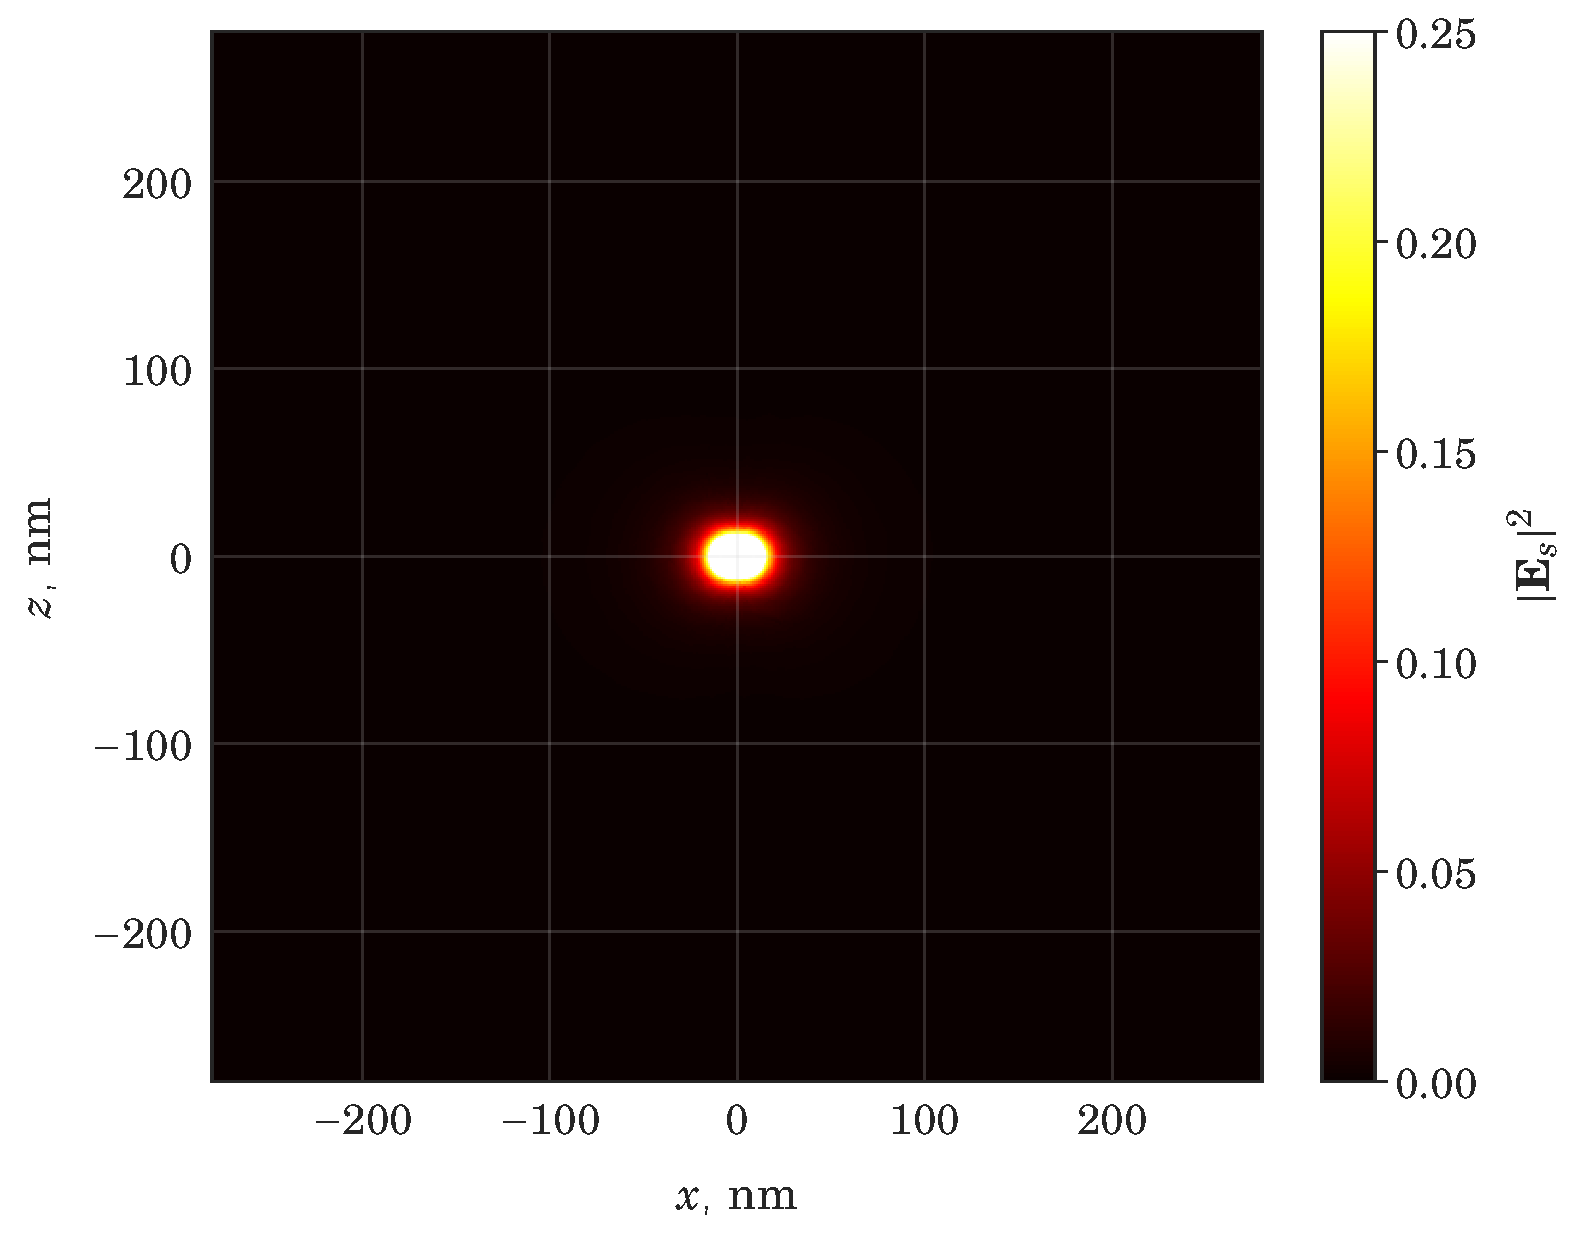
\includegraphics[width=0.45\linewidth]{../components/img/mph_new/es_ka0.7_1harm}
        }
        \hfil
        \subcaptionbox{$\lambda = \lambda_{10} = 83$ nm.}{
            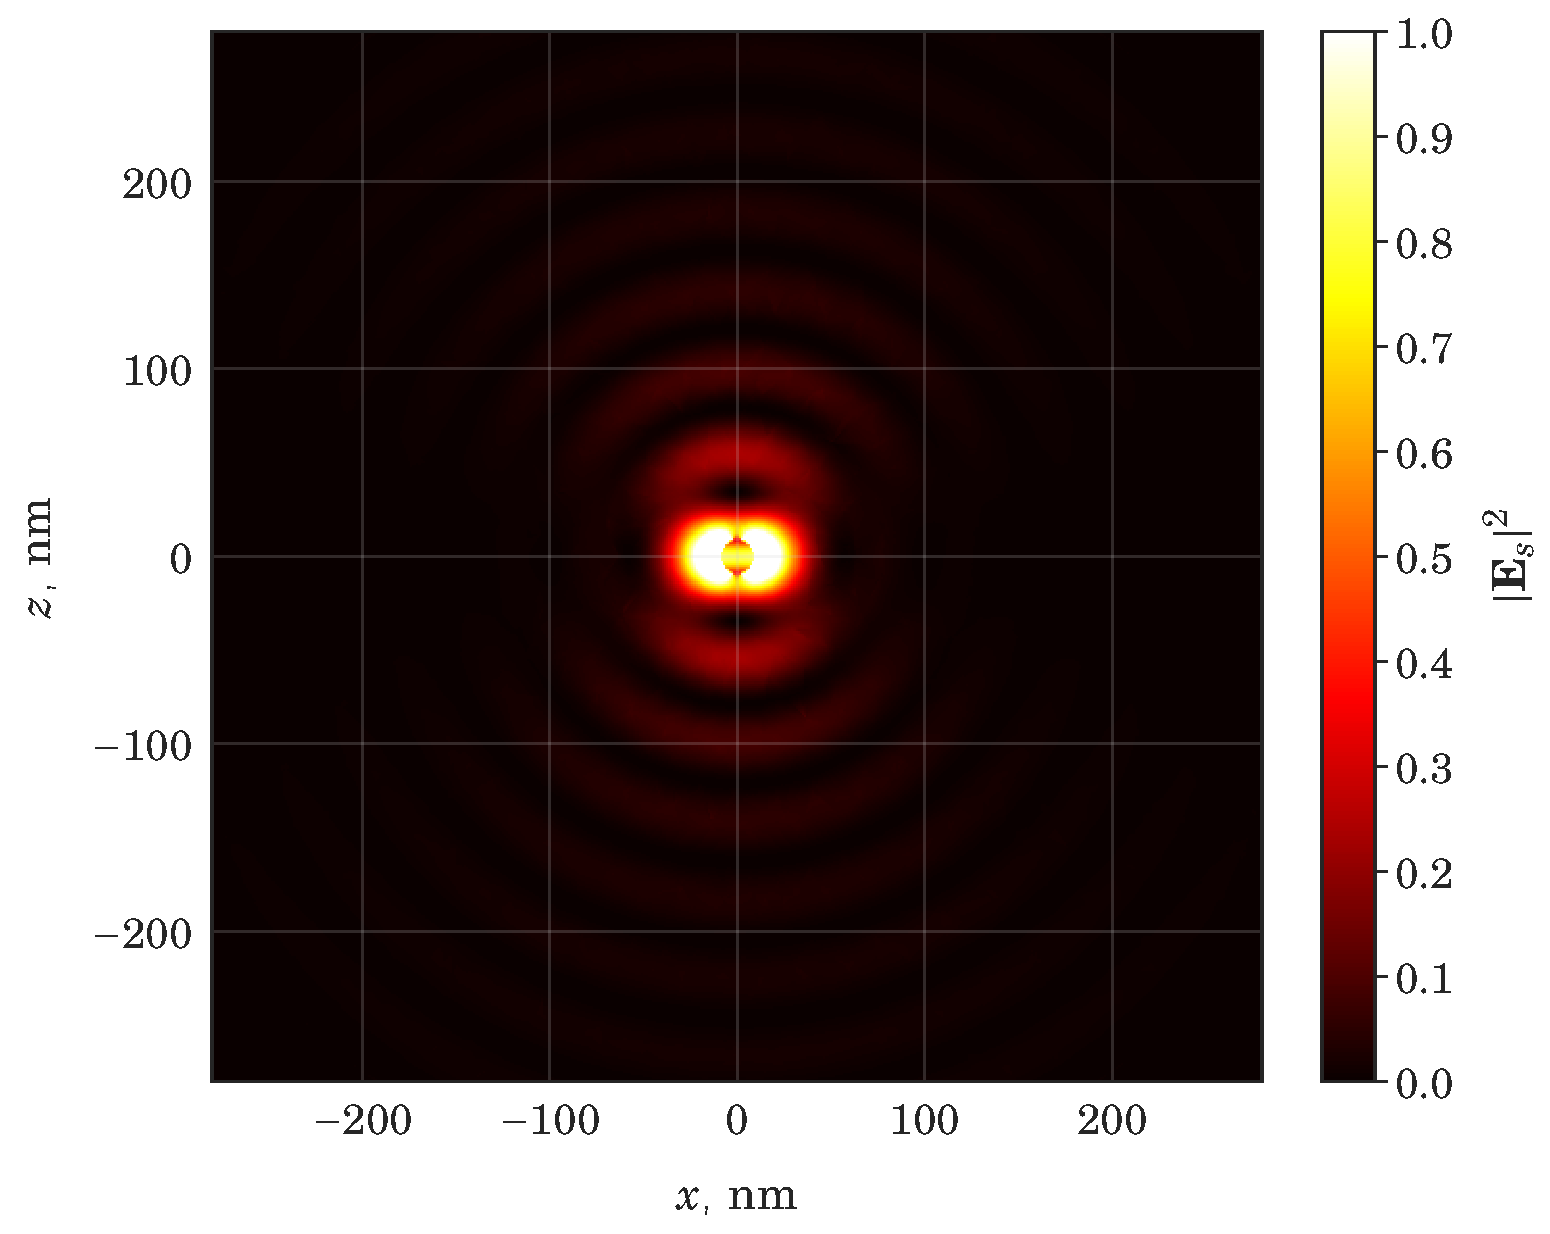
\includegraphics[width=0.45\linewidth]{../components/img/mph_new/es_ka0.7_10harm}
        }
        \label{ka0.7:image}\caption{$ka = 0.7$ ($a \approx 8.9$ nm); $|\vectbf{E}{s}|^2$ in the plane of polarization of the incident wave.}
    \end{tikzfigure}

For this case, the scattered electric field (\ref{E_s_sph}) was calculated for $\lambda = \lambda_{L}$ and $\lambda = \lambda_{10}$ in order to compare the resonant and nonresonant cases. In the resonance case the scattered field amplitude near the cluster is much higher than in the absence of resonance, where scattered waves as such are practically not observed.